\section{Teorema Fondamentale di Omomorfismi per Insiemi}
\subsection{Premessa del Teorema Fondamentale di Omomorfismo per Insiemi}
\bottom{
    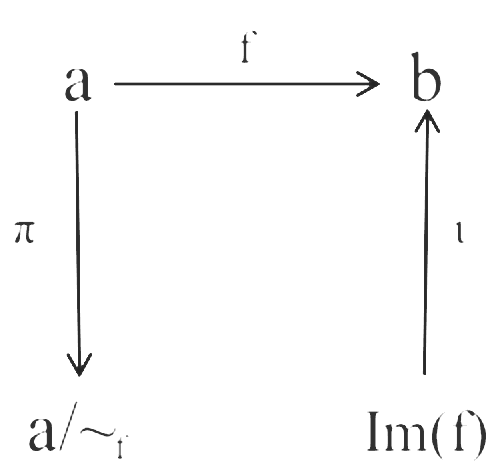
\includegraphics[scale=.2]{img/tfo1.png}

    Dati due insiemi $a$ e $b$ ed un'applicazione $f: a \to b$, possiamo costruire il seguente diagramma, dove $\pi$ è la proiezione canonica rispetto al nucleo di equivalenza di $f$ e $\iota$ (iota) è l'immersione dell'immagine nel codominio. 

    Vogliamo chiudere il diagramma, dunque definiamo:
    $$\tilde f: [x]_{\sim_f} \in a / \sim_{f}\ \mapsto\ f(x) \in Im(f)$$
    $\tilde f$ è una funzione ben posta o solo una corrispondenza? Per essere un'applicazione, per ogni classe di equivalenza deve esistere una sola immagine. Se quindi il valore $\tilde f([x]_{\sim_f})$ variasse in base a quale $z \in [x]_{\sim_f}$ scegliessimo, non sarebbe un'applicazione. Ma per definizione di nucleo di equivalenza:
    $$\forall [x]_{\sim_f} \in a / \sim_f\ \forall z, w \in [x]_{\sim_f}\ (f(z) = f(w))$$
    Allora si ha che tutti gli elementi della classe di equivalenza hanno la stessa immagine per $f$ e dunque $\tilde f$ è un'applicazione ben posta. Possiamo quindi chiudere il diagramma:

    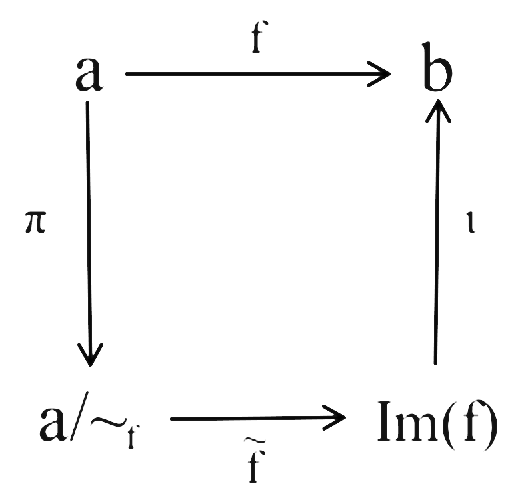
\includegraphics[scale=.2]{img/tfo2.png}
}

\subsection{Prima tesi del Teorema Fondamentale di Omomorfismi per Insiemi}
\bottom{
    $$\tilde f: [x]_{\sim_f} \in a / \sim_{f}\ \mapsto\ f(x) \in Im(f) \text{ è biettiva} $$
}
\bottomp{
    Definiamo $$\alpha: f(x) \in Im(f) \mapsto [x]_{\sim_f} \in a/\sim_f$$
    Questa è una funzione ben posta per la definizione di nucleo di equivalenza, in quanto tutte le $x$ con la stessa $f(x)$ fanno parte della stessa classe di equivalenza.
    Sia $y \in a/\sim_f$. Per le proprietà fondamentali delle classi di equivalenza $$\exists x \in a\ (y = [x]_{\sim_f})$$
    Per tanto $\alpha$ è suriettiva.

    Dalla definizione di nucleo di equivalenza $\tilde f$
    $$\forall x, y \in a\ (f(x) = f(y) \iff [x]_{\sim_f} = [y]_{\sim_f})$$
    Pertanto $\alpha$ è iniettiva.

    $\alpha$ è biettiva, $\tilde f$ è la sua inversa, quindi è anch'essa biettiva.
}

\subsection{Seconda tesi del Teorema Fondamentale di Omomorfismi per Insiemi}
\bottom{
    $$f = \iota \circ \tilde f \circ \pi$$
}
\bottomp{
    Due funzioni coincidono se hanno stesso dominio, stesso codominio, e stesso grafico.
    $$f: a \to b$$
    $$\iota \circ \tilde f \circ \pi: a\ \to\ a/\sim_f \to Im(f)\ \to\ b$$
    Hanno stesso dominio e codominio.
    $$\forall x \in a\ (\iota \circ \tilde f \circ \pi(x) = \iota(\tilde f(\pi(x))) = \iota(\tilde f([x]_{\sim_f})) = \iota(f(x)) = f(x))$$
    Anche i grafici sono identici e dunque le due funzioni sono coincidenti.
}

\subsection{Ogni Funzione è Composizione di una Funzione Iniettiva e di una Funzione Suriettiva}
\bottomp{
    Dalla $2^a$ Tesi del Teorema Fondamentale di Omomorfismo per Insiemi:
    $$\forall f\ (f = \iota \circ \tilde f \circ \pi)$$

    \(\iota\) è iniettiva, \(\tilde f\) è biettiva, e \(\pi\) è suriettiva. Pertanto possiamo esprimere \(f = (\iota \circ \tilde f) \circ \pi\) oppure \(f = \iota \circ (\tilde f \circ \pi)\). In entrambi i casi abbiamo la tesi.
}
